% Options for packages loaded elsewhere
% Options for packages loaded elsewhere
\PassOptionsToPackage{unicode}{hyperref}
\PassOptionsToPackage{hyphens}{url}
\PassOptionsToPackage{dvipsnames,svgnames,x11names}{xcolor}
%
\documentclass[
  letterpaper,
]{article}
\usepackage{xcolor}
\usepackage{amsmath,amssymb}
\setcounter{secnumdepth}{5}
\usepackage{iftex}
\ifPDFTeX
  \usepackage[T1]{fontenc}
  \usepackage[utf8]{inputenc}
  \usepackage{textcomp} % provide euro and other symbols
\else % if luatex or xetex
  \usepackage{unicode-math} % this also loads fontspec
  \defaultfontfeatures{Scale=MatchLowercase}
  \defaultfontfeatures[\rmfamily]{Ligatures=TeX,Scale=1}
\fi
\usepackage{lmodern}
\ifPDFTeX\else
  % xetex/luatex font selection
\fi
% Use upquote if available, for straight quotes in verbatim environments
\IfFileExists{upquote.sty}{\usepackage{upquote}}{}
\IfFileExists{microtype.sty}{% use microtype if available
  \usepackage[]{microtype}
  \UseMicrotypeSet[protrusion]{basicmath} % disable protrusion for tt fonts
}{}
\makeatletter
\@ifundefined{KOMAClassName}{% if non-KOMA class
  \IfFileExists{parskip.sty}{%
    \usepackage{parskip}
  }{% else
    \setlength{\parindent}{0pt}
    \setlength{\parskip}{6pt plus 2pt minus 1pt}}
}{% if KOMA class
  \KOMAoptions{parskip=half}}
\makeatother
% Make \paragraph and \subparagraph free-standing
\makeatletter
\ifx\paragraph\undefined\else
  \let\oldparagraph\paragraph
  \renewcommand{\paragraph}{
    \@ifstar
      \xxxParagraphStar
      \xxxParagraphNoStar
  }
  \newcommand{\xxxParagraphStar}[1]{\oldparagraph*{#1}\mbox{}}
  \newcommand{\xxxParagraphNoStar}[1]{\oldparagraph{#1}\mbox{}}
\fi
\ifx\subparagraph\undefined\else
  \let\oldsubparagraph\subparagraph
  \renewcommand{\subparagraph}{
    \@ifstar
      \xxxSubParagraphStar
      \xxxSubParagraphNoStar
  }
  \newcommand{\xxxSubParagraphStar}[1]{\oldsubparagraph*{#1}\mbox{}}
  \newcommand{\xxxSubParagraphNoStar}[1]{\oldsubparagraph{#1}\mbox{}}
\fi
\makeatother

\usepackage{color}
\usepackage{fancyvrb}
\newcommand{\VerbBar}{|}
\newcommand{\VERB}{\Verb[commandchars=\\\{\}]}
\DefineVerbatimEnvironment{Highlighting}{Verbatim}{commandchars=\\\{\}}
% Add ',fontsize=\small' for more characters per line
\usepackage{framed}
\definecolor{shadecolor}{RGB}{241,243,245}
\newenvironment{Shaded}{\begin{snugshade}}{\end{snugshade}}
\newcommand{\AlertTok}[1]{\textcolor[rgb]{0.68,0.00,0.00}{#1}}
\newcommand{\AnnotationTok}[1]{\textcolor[rgb]{0.37,0.37,0.37}{#1}}
\newcommand{\AttributeTok}[1]{\textcolor[rgb]{0.40,0.45,0.13}{#1}}
\newcommand{\BaseNTok}[1]{\textcolor[rgb]{0.68,0.00,0.00}{#1}}
\newcommand{\BuiltInTok}[1]{\textcolor[rgb]{0.00,0.23,0.31}{#1}}
\newcommand{\CharTok}[1]{\textcolor[rgb]{0.13,0.47,0.30}{#1}}
\newcommand{\CommentTok}[1]{\textcolor[rgb]{0.37,0.37,0.37}{#1}}
\newcommand{\CommentVarTok}[1]{\textcolor[rgb]{0.37,0.37,0.37}{\textit{#1}}}
\newcommand{\ConstantTok}[1]{\textcolor[rgb]{0.56,0.35,0.01}{#1}}
\newcommand{\ControlFlowTok}[1]{\textcolor[rgb]{0.00,0.23,0.31}{\textbf{#1}}}
\newcommand{\DataTypeTok}[1]{\textcolor[rgb]{0.68,0.00,0.00}{#1}}
\newcommand{\DecValTok}[1]{\textcolor[rgb]{0.68,0.00,0.00}{#1}}
\newcommand{\DocumentationTok}[1]{\textcolor[rgb]{0.37,0.37,0.37}{\textit{#1}}}
\newcommand{\ErrorTok}[1]{\textcolor[rgb]{0.68,0.00,0.00}{#1}}
\newcommand{\ExtensionTok}[1]{\textcolor[rgb]{0.00,0.23,0.31}{#1}}
\newcommand{\FloatTok}[1]{\textcolor[rgb]{0.68,0.00,0.00}{#1}}
\newcommand{\FunctionTok}[1]{\textcolor[rgb]{0.28,0.35,0.67}{#1}}
\newcommand{\ImportTok}[1]{\textcolor[rgb]{0.00,0.46,0.62}{#1}}
\newcommand{\InformationTok}[1]{\textcolor[rgb]{0.37,0.37,0.37}{#1}}
\newcommand{\KeywordTok}[1]{\textcolor[rgb]{0.00,0.23,0.31}{\textbf{#1}}}
\newcommand{\NormalTok}[1]{\textcolor[rgb]{0.00,0.23,0.31}{#1}}
\newcommand{\OperatorTok}[1]{\textcolor[rgb]{0.37,0.37,0.37}{#1}}
\newcommand{\OtherTok}[1]{\textcolor[rgb]{0.00,0.23,0.31}{#1}}
\newcommand{\PreprocessorTok}[1]{\textcolor[rgb]{0.68,0.00,0.00}{#1}}
\newcommand{\RegionMarkerTok}[1]{\textcolor[rgb]{0.00,0.23,0.31}{#1}}
\newcommand{\SpecialCharTok}[1]{\textcolor[rgb]{0.37,0.37,0.37}{#1}}
\newcommand{\SpecialStringTok}[1]{\textcolor[rgb]{0.13,0.47,0.30}{#1}}
\newcommand{\StringTok}[1]{\textcolor[rgb]{0.13,0.47,0.30}{#1}}
\newcommand{\VariableTok}[1]{\textcolor[rgb]{0.07,0.07,0.07}{#1}}
\newcommand{\VerbatimStringTok}[1]{\textcolor[rgb]{0.13,0.47,0.30}{#1}}
\newcommand{\WarningTok}[1]{\textcolor[rgb]{0.37,0.37,0.37}{\textit{#1}}}

\usepackage{longtable,booktabs,array}
\newcounter{none} % for unnumbered tables
\usepackage{calc} % for calculating minipage widths
% Correct order of tables after \paragraph or \subparagraph
\usepackage{etoolbox}
\makeatletter
\patchcmd\longtable{\par}{\if@noskipsec\mbox{}\fi\par}{}{}
\makeatother
% Allow footnotes in longtable head/foot
\IfFileExists{footnotehyper.sty}{\usepackage{footnotehyper}}{\usepackage{footnote}}
\makesavenoteenv{longtable}
\usepackage{graphicx}
\makeatletter
\newsavebox\pandoc@box
\newcommand*\pandocbounded[1]{% scales image to fit in text height/width
  \sbox\pandoc@box{#1}%
  \Gscale@div\@tempa{\textheight}{\dimexpr\ht\pandoc@box+\dp\pandoc@box\relax}%
  \Gscale@div\@tempb{\linewidth}{\wd\pandoc@box}%
  \ifdim\@tempb\p@<\@tempa\p@\let\@tempa\@tempb\fi% select the smaller of both
  \ifdim\@tempa\p@<\p@\scalebox{\@tempa}{\usebox\pandoc@box}%
  \else\usebox{\pandoc@box}%
  \fi%
}
% Set default figure placement to htbp
\def\fps@figure{htbp}
\makeatother





\setlength{\emergencystretch}{3em} % prevent overfull lines

\providecommand{\tightlist}{%
  \setlength{\itemsep}{0pt}\setlength{\parskip}{0pt}}



 


\makeatletter
\@ifpackageloaded{caption}{}{\usepackage{caption}}
\AtBeginDocument{%
\ifdefined\contentsname
  \renewcommand*\contentsname{Table of contents}
\else
  \newcommand\contentsname{Table of contents}
\fi
\ifdefined\listfigurename
  \renewcommand*\listfigurename{List of Figures}
\else
  \newcommand\listfigurename{List of Figures}
\fi
\ifdefined\listtablename
  \renewcommand*\listtablename{List of Tables}
\else
  \newcommand\listtablename{List of Tables}
\fi
\ifdefined\figurename
  \renewcommand*\figurename{Figure}
\else
  \newcommand\figurename{Figure}
\fi
\ifdefined\tablename
  \renewcommand*\tablename{Table}
\else
  \newcommand\tablename{Table}
\fi
}
\@ifpackageloaded{float}{}{\usepackage{float}}
\floatstyle{ruled}
\@ifundefined{c@chapter}{\newfloat{codelisting}{h}{lop}}{\newfloat{codelisting}{h}{lop}[chapter]}
\floatname{codelisting}{Listing}
\newcommand*\listoflistings{\listof{codelisting}{List of Listings}}
\makeatother
\makeatletter
\makeatother
\makeatletter
\@ifpackageloaded{caption}{}{\usepackage{caption}}
\@ifpackageloaded{subcaption}{}{\usepackage{subcaption}}
\makeatother
\usepackage{bookmark}
\IfFileExists{xurl.sty}{\usepackage{xurl}}{} % add URL line breaks if available
\urlstyle{same}
\hypersetup{
  pdftitle={Desafio 01: Elementos de Aprendizado de Máquina},
  pdfauthor={Lorrayne Silva; Kammyla Landim; Paulo Emílio Silva Vaz},
  colorlinks=true,
  linkcolor={blue},
  filecolor={Maroon},
  citecolor={Blue},
  urlcolor={Blue},
  pdfcreator={LaTeX via pandoc}}


\title{Desafio 01: Elementos de Aprendizado de Máquina}
\usepackage{etoolbox}
\makeatletter
\providecommand{\subtitle}[1]{% add subtitle to \maketitle
  \apptocmd{\@title}{\par {\large #1 \par}}{}{}
}
\makeatother
\subtitle{Análise de Regressão de Poisson - Dataset Danish Lung Cancer}
\author{Lorrayne Silva \and Kammyla Landim \and Paulo Emílio Silva Vaz}
\date{2026-05-11}
\begin{document}
\maketitle

\renewcommand*\contentsname{Table of contents}
{
\setcounter{tocdepth}{3}
\tableofcontents
}

\section{Questão 1: Carga, Preparação e Análise Descritiva dos
Dados}\label{questuxe3o-1-carga-preparauxe7uxe3o-e-anuxe1lise-descritiva-dos-dados}

\begin{Shaded}
\begin{Highlighting}[]
\CommentTok{\# Criando o data frame com os dados do desafio}
\NormalTok{danishlc }\OtherTok{\textless{}{-}} \FunctionTok{data.frame}\NormalTok{(}
  \AttributeTok{City =} \FunctionTok{rep}\NormalTok{(}\FunctionTok{c}\NormalTok{(}\StringTok{"Fredericia"}\NormalTok{, }\StringTok{"Horsens"}\NormalTok{, }\StringTok{"Kolding"}\NormalTok{, }\StringTok{"Vejle"}\NormalTok{), }\AttributeTok{each =} \DecValTok{5}\NormalTok{),}
  \AttributeTok{Age =} \FunctionTok{rep}\NormalTok{(}\FunctionTok{c}\NormalTok{(}\StringTok{"40{-}54"}\NormalTok{, }\StringTok{"55{-}59"}\NormalTok{, }\StringTok{"60{-}64"}\NormalTok{, }\StringTok{"65{-}74"}\NormalTok{, }\StringTok{"\textgreater{}74"}\NormalTok{), }\AttributeTok{times =} \DecValTok{4}\NormalTok{),}
  \AttributeTok{Pop =} \FunctionTok{c}\NormalTok{(}\DecValTok{3059}\NormalTok{, }\DecValTok{800}\NormalTok{, }\DecValTok{710}\NormalTok{, }\DecValTok{581}\NormalTok{, }\DecValTok{509}\NormalTok{,  }
          \DecValTok{3083}\NormalTok{, }\DecValTok{712}\NormalTok{, }\DecValTok{625}\NormalTok{, }\DecValTok{402}\NormalTok{, }\DecValTok{290}\NormalTok{,  }
          \DecValTok{2867}\NormalTok{, }\DecValTok{597}\NormalTok{, }\DecValTok{526}\NormalTok{, }\DecValTok{350}\NormalTok{, }\DecValTok{223}\NormalTok{,  }
          \DecValTok{2914}\NormalTok{, }\DecValTok{539}\NormalTok{, }\DecValTok{461}\NormalTok{, }\DecValTok{307}\NormalTok{, }\DecValTok{189}\NormalTok{),}
  \AttributeTok{Cases =} \FunctionTok{c}\NormalTok{(}\DecValTok{11}\NormalTok{, }\DecValTok{11}\NormalTok{, }\DecValTok{11}\NormalTok{, }\DecValTok{10}\NormalTok{, }\DecValTok{11}\NormalTok{,  }
            \DecValTok{15}\NormalTok{, }\DecValTok{6}\NormalTok{, }\DecValTok{8}\NormalTok{, }\DecValTok{7}\NormalTok{, }\DecValTok{4}\NormalTok{,  }
            \DecValTok{11}\NormalTok{, }\DecValTok{13}\NormalTok{, }\DecValTok{9}\NormalTok{, }\DecValTok{11}\NormalTok{, }\DecValTok{10}\NormalTok{,  }
            \DecValTok{10}\NormalTok{, }\DecValTok{8}\NormalTok{, }\DecValTok{7}\NormalTok{, }\DecValTok{10}\NormalTok{, }\DecValTok{14}\NormalTok{)}
\NormalTok{)}

\CommentTok{\# Convertendo as variáveis explicativas para fatores}
\NormalTok{danishlc}\SpecialCharTok{$}\NormalTok{City }\OtherTok{\textless{}{-}} \FunctionTok{as.factor}\NormalTok{(danishlc}\SpecialCharTok{$}\NormalTok{City)}
\NormalTok{danishlc}\SpecialCharTok{$}\NormalTok{Age }\OtherTok{\textless{}{-}} \FunctionTok{as.factor}\NormalTok{(danishlc}\SpecialCharTok{$}\NormalTok{Age)}

\CommentTok{\# Calculando a Taxa Bruta de Incidência (por 1.000 habitantes)}
\NormalTok{danishlc}\SpecialCharTok{$}\NormalTok{Taxa }\OtherTok{\textless{}{-}}\NormalTok{ (danishlc}\SpecialCharTok{$}\NormalTok{Cases }\SpecialCharTok{/}\NormalTok{ danishlc}\SpecialCharTok{$}\NormalTok{Pop) }\SpecialCharTok{*} \DecValTok{1000}

\CommentTok{\# Visualizando o sumário descritivo dos dados}
\FunctionTok{summary}\NormalTok{(danishlc)}
\end{Highlighting}
\end{Shaded}

\begin{verbatim}
         City      Age         Pop             Cases            Taxa       
 Fredericia:5   >74  :4   Min.   : 189.0   Min.   : 4.00   Min.   : 3.432  
 Horsens   :5   40-54:4   1st Qu.: 389.0   1st Qu.: 8.00   1st Qu.:11.707  
 Kolding   :5   55-59:4   Median : 560.0   Median :10.00   Median :15.339  
 Vejle     :5   60-64:4   Mean   : 987.2   Mean   : 9.85   Mean   :19.403  
                65-74:4   3rd Qu.: 734.0   3rd Qu.:11.00   3rd Qu.:21.652  
                          Max.   :3083.0   Max.   :15.00   Max.   :74.074  
\end{verbatim}

\begin{Shaded}
\begin{Highlighting}[]
\FunctionTok{library}\NormalTok{(ggplot2)}

\FunctionTok{ggplot}\NormalTok{(danishlc, }\FunctionTok{aes}\NormalTok{(}\AttributeTok{x =}\NormalTok{ Age, }\AttributeTok{y =}\NormalTok{ Taxa, }\AttributeTok{fill =}\NormalTok{ City)) }\SpecialCharTok{+}
  \FunctionTok{geom\_bar}\NormalTok{(}\AttributeTok{stat =} \StringTok{"identity"}\NormalTok{, }\AttributeTok{position =} \StringTok{"dodge"}\NormalTok{) }\SpecialCharTok{+}
  \FunctionTok{theme\_minimal}\NormalTok{() }\SpecialCharTok{+}
  \FunctionTok{labs}\NormalTok{(}
    \AttributeTok{title =} \StringTok{"Taxa de Incidência de Câncer de Pulmão por 1.000 Habitantes"}\NormalTok{,}
    \AttributeTok{x =} \StringTok{"Faixa Etária (Anos)"}\NormalTok{,}
    \AttributeTok{y =} \StringTok{"Casos por 1.000 Habitantes"}\NormalTok{,}
    \AttributeTok{fill =} \StringTok{"Cidade"}
\NormalTok{  ) }\SpecialCharTok{+}
  \FunctionTok{scale\_fill\_brewer}\NormalTok{(}\AttributeTok{palette =} \StringTok{"Set2"}\NormalTok{)}
\end{Highlighting}
\end{Shaded}

\begin{center}
\pandocbounded{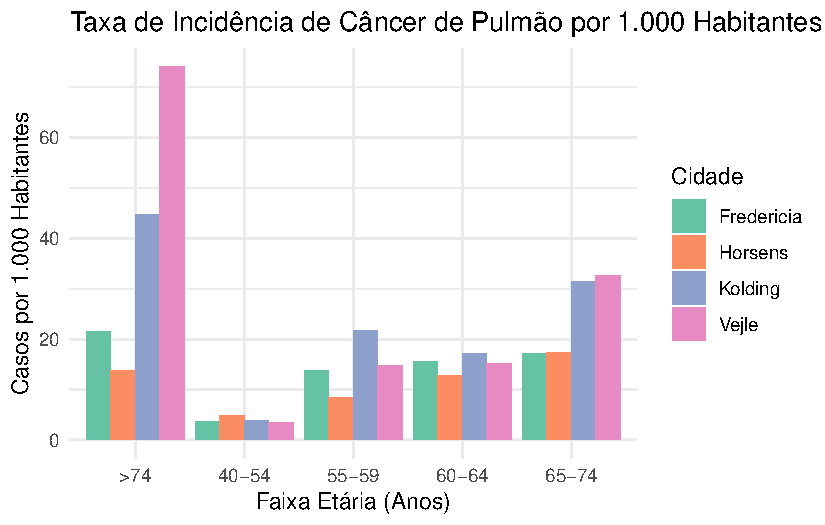
\includegraphics[keepaspectratio]{Desafio-01_files/figure-pdf/unnamed-chunk-1-1.pdf}}
\end{center}

\begin{Shaded}
\begin{Highlighting}[]
\CommentTok{\# Ajustando o modelo de Poisson com offset populacional}
\NormalTok{modelo\_poisson }\OtherTok{\textless{}{-}} \FunctionTok{glm}\NormalTok{(}
\NormalTok{  Cases }\SpecialCharTok{\textasciitilde{}}\NormalTok{ City }\SpecialCharTok{+}\NormalTok{ Age, }
  \AttributeTok{family =} \FunctionTok{poisson}\NormalTok{(}\AttributeTok{link =} \StringTok{"log"}\NormalTok{), }
  \AttributeTok{offset =} \FunctionTok{log}\NormalTok{(Pop), }
  \AttributeTok{data =}\NormalTok{ danishlc}
\NormalTok{)}

\CommentTok{\# Exibindo os resultados detalhados do modelo}
\FunctionTok{summary}\NormalTok{(modelo\_poisson)}
\end{Highlighting}
\end{Shaded}

\begin{verbatim}

Call:
glm(formula = Cases ~ City + Age, family = poisson(link = "log"), 
    data = danishlc, offset = log(Pop))

Coefficients:
            Estimate Std. Error z value Pr(>|z|)    
(Intercept) -3.57882    0.19004 -18.832  < 2e-16 ***
CityHorsens -0.05664    0.20918  -0.271 0.786564    
CityKolding  0.40221    0.19339   2.080 0.037543 *  
CityVejle    0.39649    0.19865   1.996 0.045945 *  
Age40-54    -2.15918    0.21821  -9.895  < 2e-16 ***
Age55-59    -0.84403    0.22867  -3.691 0.000223 ***
Age60-64    -0.79328    0.23350  -3.397 0.000680 ***
Age65-74    -0.35432    0.22821  -1.553 0.120509    
---
Signif. codes:  0 '***' 0.001 '**' 0.01 '*' 0.05 '.' 0.1 ' ' 1

(Dispersion parameter for poisson family taken to be 1)

    Null deviance: 147.943  on 19  degrees of freedom
Residual deviance:  14.484  on 12  degrees of freedom
AIC: 112.55

Number of Fisher Scoring iterations: 4
\end{verbatim}

\begin{verbatim}
#| message: false
#| warning: false

# Extraindo as razões de taxas (exponencial dos coeficientes)
razao_taxas <- exp(coef(modelo_poisson))

# Calculando os Intervalos de Confiança (95%)
ic_razao_taxas <- exp(confint(modelo_poisson))

# Consolidando os resultados em uma tabela
tabela_interpretacao <- cbind(
  `Razão de Taxas (RR)` = razao_taxas, 
  ic_razao_taxas
)

print(round(tabela_interpretacao, 4))}
\end{verbatim}

\begin{verbatim}
#| message: false
#| warning: false

# Extraindo estatísticas de ajuste
deviance_residual <- modelo_poisson$deviance
graus_liberdade <- modelo_poisson$df.residual

# Calculando o p-valor do teste Qui-Quadrado
p_valor_ajuste <- pchisq(deviance_residual, df = graus_liberdade, lower.tail = FALSE)

cat("Deviance Residual:", round(deviance_residual, 4), "\n")
cat("Graus de Liberdade:", graus_liberdade, "\n")
cat("P-valor do Teste de Ajuste:", round(p_valor_ajuste, 4), "\n")
\end{verbatim}




\end{document}
